%%%%%%%%%%%%%%%%%%%%%%%%%%%%%%%%%%%%%%%%%
% Beamer Presentation
% LaTeX Template
% Version 1.0 (10/11/12)
%
% This template has been downloaded from:
% http://www.LaTeXTemplates.com
%
% License:
% CC BY-NC-SA 3.0 (http://creativecommons.org/licenses/by-nc-sa/3.0/)
%
%%%%%%%%%%%%%%%%%%%%%%%%%%%%%%%%%%%%%%%%%

%----------------------------------------------------------------------------------------
%	PACKAGES AND THEMES
%----------------------------------------------------------------------------------------
\documentclass[fontset=windows,12pt,t,aspectratio=169]{beamer}
\mode<presentation> {
% The Beamer class comes with a number of default slide themes
% which change the colors and layouts of slides. Below this is a list
% of all the themes, uncomment each in turn to see what they look like.

%\usetheme{default}
%\usetheme{AnnArbor}
%\usetheme{Antibes}
%\usetheme{Bergen}
%\usetheme{Berkeley}
%\usetheme{Berlin}
%\usetheme{Boadilla}
\usetheme{CambridgeUS}
%\usetheme{Copenhagen}
%\usetheme{Darmstadt}
%\usetheme{Dresden}
%\usetheme{Frankfurt}
%\usetheme{Goettingen}
%\usetheme{Hannover}
%\usetheme{Ilmenau}
%\usetheme{JuanLesPins}
%\usetheme{Luebeck}
%\usetheme{Madrid}
%\usetheme{Malmoe}
%\usetheme{Marburg}
%\usetheme{Montpellier}
%\usetheme{PaloAlto}
%\usetheme{Pittsburgh}
%\usetheme{Rochester}
%\usetheme{Singapore}
%\usetheme{Szeged}
%\usetheme{Warsaw}

% As well as themes, the Beamer class has a number of color themes
% for any slide theme. Uncomment each of these in turn to see how it
% changes the colors of your current slide theme.

%\usecolortheme{albatross}
%\usecolortheme{beaver}
%\usecolortheme{beetle}
%\usecolortheme{crane}
%\usecolortheme{dolphin}
%\usecolortheme{dove}
%\usecolortheme{fly}
%\usecolortheme{lily}
%\usecolortheme{orchid}
%\usecolortheme{rose}
%\usecolortheme{seagull}
%\usecolortheme{seahorse}
%\usecolortheme{whale}
%\usecolortheme{wolverine}

%\setbeamertemplate{footline} % To remove the footer line in all slides uncomment this line
%\setbeamertemplate{footline}[page number] % To replace the footer line in all slides with a simple slide count uncomment this line

%\setbeamertemplate{navigation symbols}{} % To remove the navigation symbols from the bottom of all slides uncomment this line
}


\usepackage[UTF8]{ctex}
%\usepackage{fontspec}
%\usepackage{xeCJK}


% 设置中文字体
%\setCJKmainfont{SIMSUN.TTC} % 替换为你系统中宋体的名称
%\setbeamerfont{normal text}{family=宋体}
%\setmainfont{SIMSUN.TTC}

%\setbeamercolor{normal text}{fg=foreground,bg=background}
%设置标题、目录和页眉页脚
%\setbeamercolor{author in head/foot}{fg=white, bg=shenhong}
%\setbeamercolor{title in head/foot}{fg=black, bg=weibai}  %bg页脚颜色
%\setbeamercolor{date in head/foot}{fg=black, bg=huise} %设置日期颜色

%\setbeamercolor{institute}{fg=black} %设置机构颜色
%\setbeamercolor{item}{fg=blue}  %设置目录序号颜色
%二级目录
%\setbeamercolor{subitem}{fg=dblue} %设置二级目录序号颜色
%\setbeamercolor{itemize/enumerate subbody}{fg=black} %设置二级目录文字颜色
%\setbeamertemplate{itemize subitem}{{circle}} %设置二级目录符号为短线(\textendash) \textbullet是文本模式下的圆点符号,而\bullet通常用于数学模式
%\setbeamerfont{itemize/enumerate subbody}{size=\footnotesize} %设置二级目录字体small footnotesize normalsize
%\setbeamerfont{itemize/enumerate subitem}{size=\footnotesize}

%\setbeamertemplate{itemize items}[circle] % 设置圆点符号
%\setbeamertemplate{enumerate items}[default] % 设置编号样式


\usepackage{graphicx} % Allows including images
\usepackage{booktabs} % Allows the use of \toprule, \midrule and \bottomrule in tables
\usepackage[justification=centering]{caption} %调整图表标题的格式。在这里,通过 justification=centering 设置标题居中对齐
\usepackage {subcaption} %该宏包允许你创建并排的子图
\usepackage{multicol}  %用于创建多列布局。在这个环境中,文本和其他内容可以自动分布到多个列中。
\usepackage{amsmath}  %它扩展了 LaTeX 的数学功能,提供了一些额外的数学符号、结构和环境。其中,align 等环境允许多行公式的对齐



%\usepackage[nameinlink]{cleveref} %引用图表显示Figure

\setbeamertemplate{caption}[numbered]  %图表显示编号
%\crefname{figure}{Figure}{Figures}  %\cref引用自己定义的名字
%\Crefname{figure}{Figure}{Figures}
%\definecolor{shenhong}{RGB}{170,0,0}
%\setbeamercolor{titlelike}{fg=white,bg=shenhong}  %设置标题框颜色(最上面和第一页标题框)
%\setbeamercolor{frametitle}{fg=white,bg=shenhong} %设置子标题颜色


%----------------------------------------------------------------------------------------
%	TITLE PAGE
%----------------------------------------------------------------------------------------

\title[The role of inventories and capacity utilization]{The role of inventories and capacity utilization as shock absorbers} % The short title appears at the bottom of every slide, the full title is only on the title page

\author[\emph{Leonardo Auernheimer, Danilo R. Trupkin}]{\emph{Leonardo Auernheimer, Danilo R. Trupkin}}
\institute[] {
Review of Economic Dynamics 17 (2014) 70–85\medskip

\normalsize 十三组: 刘方; 张全飞; 王珂辉; 刘淙; 耿宁; 周荣耀% Your institution for the title page
}
\date {2023/12}

\begin{document} {
    \setbeamertemplate{footline}{}
    \frame {
        \titlepage
    }
}

\pgfdeclareimage[height=1cm]{logo}{sdu.jpg}
\logo{\pgfuseimage{logo}}

\AtBeginSection{
  %\setbeamertemplate{headline}{} % 隐藏标题栏
  \begin{frame}[allowframebreaks]
  \frametitle{Overview}
    \tableofcontents[currentsection,currentsubsection]
  \end{frame}
  %\setbeamertemplate{headline}[default] % 恢复标题栏
}


%子节
\AtBeginSubsection{
  \begin{frame}[allowframebreaks]

  \frametitle{Overview}
    \tableofcontents[currentsection,currentsubsection]
  \end{frame}
}

%----------------------------------------------------------------------------------------
%	PRESENTATION SLIDES
%----------------------------------------------------------------------------------------


%----------------------------------------------------------------------------------------
\begin{frame}
	\begin{multicols}{2}
		\begin{figure}
			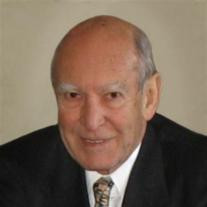
\includegraphics[height=100pt]{table/Leon.jpg}
			\caption*{Leonardo Auernheimer\\(Texas A\&M University)}
			
\includegraphics[height=100pt]{table/Danilo.png}
			\caption*{Danilo R. Trupkin \\(Universidad de Buenos Aires)}
		\end{figure}
	\end{multicols}
    \vspace{5pt}
    \begin{itemize}
      \item Leonardo's research area include monetary economics and open economy macroeconomics,and he was an associate editor of the JAE and the JDE.
      \item Danilo's research areas include monetary economics, macroeconomics and international trade.
    \end{itemize}
\end{frame}


%----------------------------------------------------------------------------------------
\section{Introduction}
%----------------------------------------------------------------------------------------
\begin{frame}{The primary goal}
 \begin{itemize}
   \item The primary goal of this paper is to analyze the role of inventories and capacity utilization – the intensity of use of both capital and labor – in the transmission of business cycle fluctuations.
   \vspace{5pt}
   \item We study the relationship between these variables and what they would respond to shocks of different rates of persistence.
   \vspace{5pt}
     \item Inventories are zero-return assets,Causes of demand for inventory:
     \vspace{5pt}
      \begin{itemize}
        \item Allows consumers either to match their tastes more effectively.
        \vspace{5pt}
        \item To economize on shopping cost.
      \end{itemize}
 \end{itemize}
\end{frame}

%----------------------------------------------------------------------------------------3
\begin{frame}{The primary result}
    \begin{figure}
         \begin{center}
         \caption*{Primary result}
         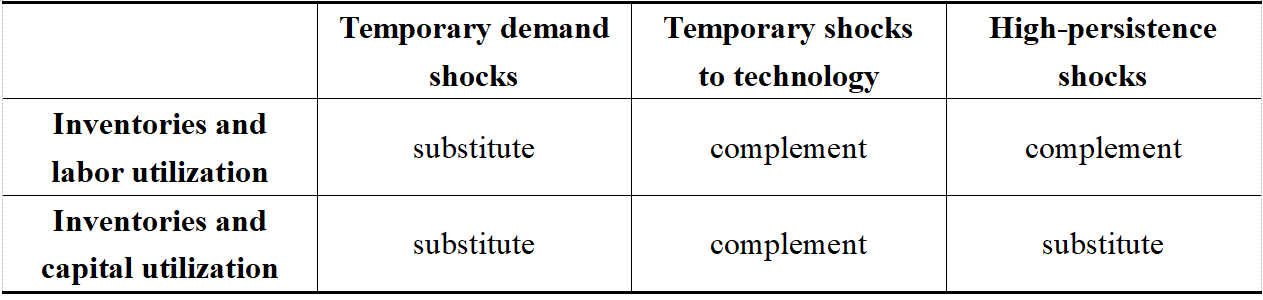
\includegraphics[width=11cm]{table/result.png}
         \end{center}
    \end{figure}
   \begin{itemize}

     \item Therefore, temporary demand shocks emphasize the role of inventories as being a “\textbf{shock absorber}”, whereas high-persistence demand shocks, emphasize the role of inventories as being a \textbf{complement to consumption}.
   \end{itemize}
\end{frame}

%----------------------------------------------------------------------------------------3
\begin{frame}{Contributes}
   \begin{itemize}
     \item Inventory and capacity utilization are both taken into account.
     \vspace{5pt}
     \item Analyze the theoretical relationship between inventory and capacity utilization and how it affects business cycle transmission.
     \vspace{5pt}
     \item DSGE model that distinguishes from earlier models:
     \begin{itemize}
       \item (i) endogenous capital depreciation
       \vspace{5pt}
       \item (ii) variable use of the labor force
       \vspace{5pt}
       \item (iii) adjustment costs in physical capital
       \vspace{5pt}
       \item (iv) inventory holdings
     \end{itemize}

   \end{itemize}
\end{frame}

%----------------------------------------------------------------------------------------
\section{The model}
%\subsection{Environment}
%----------------------------------------------------------------------------------------
\begin{frame}{Environment}
    \begin{itemize}
       \item Output:
    \end{itemize}
    \[ Y_t = \omega_t F(e_t N_t, s_t K_t) \]
    \begin{itemize}
    \item Variable definition:
        \begin{itemize}
           \item $N_t$: the levels of labor at time $t$
           \item $K_t$: the levels of capital at time $t$
           \item $e_t$: the rates of labor utilization at time $t$
           \item $s_t$: the rates of capital utilization at time $t$
           \item $\omega_t$: the exogenous, stochastic time-$t$ level of total factor productivity, assumed to follow a stationary AR(1) process
        \end{itemize}
    \end{itemize}
\end{frame}

%----------------------------------------------------------------------------------------
\begin{frame}{Environment}
    \begin{itemize}
       \item The law of motion for capital:
    \end{itemize}
    \[ K_{t+1} = K_t[1 - \delta (s_t)] + I_t\big[1 - S(\frac{I_t}{I_{t-1}})\big] \tag{1} \]
    \begin{itemize}
      \item $\delta(s_t)$ and $S(\cdot)$
        \begin{itemize}
            \item \( \delta(s_t) \): time-\(t\) depreciation rate of capital.
            \item \( S \): function representing adjustment costs in investment, satisfying \( S(1) = S'(1) = 0 \) and \( \kappa \equiv S''(1) > 0 \).
         \end{itemize}
         \item Resource constraint:
        \[ C_t + I_t + Q_{t+1} - (1 - \delta_q) Q_t \leq Y_t \tag{2} \]
    \end{itemize}
\end{frame}

%----------------------------------------------------------------------------------------
\begin{frame}{Environment}
    \begin{itemize}

        \item Expected lifetime utility:
        \[ E_0 \sum_{t=0}^{\infty} \beta^t \left[ z_t u(C_t, Q_t) + v(l_t) + w(e_t) \right]  \tag{3} \]
        \item Definition
        \begin{itemize}
            \item $l_t$: $l_t \equiv 1 - e_t N_t$, leisure at time $t$
            \item $z_t$: an exogenous, stochastic preference shock, assume that the preference (demand) shock follows a stationary AR(1) process
            \item $w(1) = 0$, $w'(e_t) > $ or $< 0$, for $e_t < $ or $> 1$, and $w''(e_t) < 0$, for all $e_t$.
            \item $u_c(\cdot) > 0, u_{cc}(\cdot) < 0; \quad u_q(\cdot) > 0, u_{qq}(\cdot) < 0; \quad v'(\cdot) > 0, v''(\cdot) \leq 0.$

        \end{itemize}
    \end{itemize}
\end{frame}

%----------------------------------------------------------------------------------------
\begin{frame}{Optimality conditions}
    \begin{itemize}
        \item The optimality condition related to labor utilization:
        \[    z_t u_c(C_t, Q_t) \omega_t F_{eN}(e_t N_t, s_t K_t) - v'(l_t) = -\frac{w'(e_t)}{N_t} \tag{6} \]
        \item  Notice that, if the decision taken at $t - 1$ with respect to ex-ante labor ($N_t$) was also optimal ex-post with new information at $t$, then the optimal utilization rate will be unity.
        \item This is the same as saying that the right-hand side of (6) becomes zero.
        \item A standard optimality condition for labor that sets the marginal rate of substitution between consumption and leisure equal to the marginal product of labor.
    \end{itemize}
\end{frame}

\setlength{\parskip}{1em}
%----------------------------------------------------------------------------------------
\begin{frame}{Questions}
    \quad  为什么效用最大化时 $e_t = 1$ ?
    \begin{itemize}
        \item 在最优状态下,一单位消费的边际效用应与一单位闲暇的边际效用相等。具体而言,增加一单位消费所带来的效用增益应与增加一单位闲暇所带来的效用增益相匹配。否则,代理人可能更倾向于选择消费或闲暇。
        \item 在这一最优状态下,若代理人受到不确定性冲击(例如加班)导致工作时间变化($e_t \neq 1$),消费增加的效用和闲暇减少的效用仍应保持相等。然而,由于代理人的行为可能产生偏离,引入了惩罚项,导致整体效用减少。因此,当$e_t = 1$时,代理人没有偏离该状态的动机,使其成为最优状态。
    \end{itemize}
\end{frame}


%----------------------------------------------------------------------------------------
\begin{frame}{Optimality conditions}
    \begin{itemize}
        \item Second, the optimality condition with respect to capital utilization is:
        \begin{equation}
        \omega_t F_{sK}(e_t N_t, s_t K_t) = \delta'(s_t) p_{k,t} \tag{7}
        \end{equation}
        \item $p_{k,t}$ is the shadow value of a unit of capital in terms of consumption, the ratio between the multiplier associated to the resource constraint and the multiplier associated to the law of motion for capital.
        \item $\delta'(s_t)$,the marginal cost in terms of a higher depreciation from using capital more intensively
        \item Efficient use of capital is that the marginal benefit of capital services equal to the marginal user's cost.
    \end{itemize}
\end{frame}

%----------------------------------------------------------------------------------------
\begin{frame}{Optimality conditions}
    \begin{itemize}
        \item Finally, the optimality condition with respect to inventory holdings:
       \[
z_t u_c(C_t, Q_t) = \beta E_t \left\{ z_{t+1} [\underline{u_c(C_{t+1}, Q_{t+1}) (1 - \delta_q)}_{\text{1}} + \underline{u_q(C_{t+1}, Q_{t+1})}_{\text{2}}] \  \vert \  \omega_t, z_t \right\} \tag{8}
\]
        \item the equation represent: the loss in current utility = the discounted expected future.
        \item the 1 on the right: its future value, equal to the value of a unit of consumption, net of inventory storage costs.
        \item the 2 on the right: the future utility received from an extra unit of inventory accumulated today.
    \end{itemize}
\end{frame}

%----------------------------------------------------------------------------------------
\section{Solving the model: Main results}
%----------------------------------------------------------------------------------------
\begin{frame}{Functional forms and calibration}
    \begin{itemize}
       \item The production technology is assumed to be:
       $$ F(e_tN_t, s_tK_t) = (e_t N_t)^{1-\alpha} (s_t K_t)^{\alpha}$$
       \item The components of the period utility function are given as follows:
       $$ u(C_t, Q_t) = \ln\left[ \theta C_t^{1-\gamma} + (1-\theta) Q_t^{1-\gamma} \right]^{\frac{1}{1-\gamma}}, v(l_t) = \eta l_t, w(e_t) = -\frac{\phi}{2}(e_t - 1)^2 $$
       \item with $\eta > 0, \quad \phi > 0, \quad 0 < \theta < 1, \quad \gamma > 1  $
       \item  $\gamma$ is the inverse of an elasticity of substitution.
       \item  $\theta$ represents the weight of consumption in the CES bundle.
    \end{itemize}
\end{frame}

%----------------------------------------------------------------------------------------
\begin{frame}{Functional forms and calibration}
    \begin{itemize}
       \item The stochastic processes for technology and preferences, are assumed to evolve according to:
        \begin{align*}
            &\ln(\omega_t) = \rho_\omega \ln(\omega_{t-1}) + \epsilon_{\omega t}, \tag{9}
            \\
            &\ln(z_t) = \rho_z \ln(z_{t-1}) + \epsilon_{zt}, \tag{10}
        \end{align*}
       \item where $0 < \rho_\omega < 1$ and $0 < \rho_z < 1$
       \item $\epsilon_{\omega t} $ and $ \epsilon_{zt} $ are serially uncorrelated random variables with zero mean and standard deviations $\sigma_\omega$ and $\sigma_z $.
    \end{itemize}
\end{frame}

%----------------------------------------------------------------------------------------
\begin{frame}{Functional forms and calibration}
    \begin{itemize}
       \item We assume that the rate of capital depreciation is given by: $\delta(s_t) = \delta s_{t}^{v} $, with \(0 < \delta < 1\), and \(v > 1\).
       \item The investment adjustment cost function as:
       \[S(\frac{I_t}{I_{t-1}}) = \frac{\kappa}{2}(\frac{I_t}{I_{t-1}} - 1)^2\]
       \item All the references to the data statistics will be based on U.S. quarterly series, 1967:1–2011:4, seasonally adjusted, except when indicated.
       \begin{figure}
         \begin{center}
         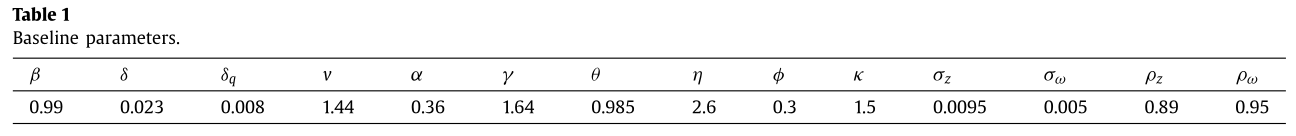
\includegraphics[width=12cm]{table/tab1.png}
         \end{center}
       \end{figure}
    \end{itemize}
\end{frame}

%----------------------------------------------------------------------------------------
\begin{frame}{Impulse–response analysis}
    \begin{itemize}
       \item  Our goal is to characterize in detail the impact effect and subsequent convergence of the economy in
response to the shocks considered.
       \item  First, to the IRFs of inventory holdings, labor utilization and capital utilization ($\rho_\omega = 0.89$ and $\rho_z = 0.95$).
       \item Afterward, we study the IRFs based on non-persistent shocks ($\rho_\omega = \rho_z = 0$).
       \item Finally, in order to characterize in detail the differences in behavior between utilization rates and capacity, we analyze the IRFs of the flow of services from labor and capital.
    \end{itemize}
\end{frame}

%----------------------------------------------------------------------------------------
\begin{frame}{Impulse–response analysis}
    \begin{figure}
         \begin{center}
         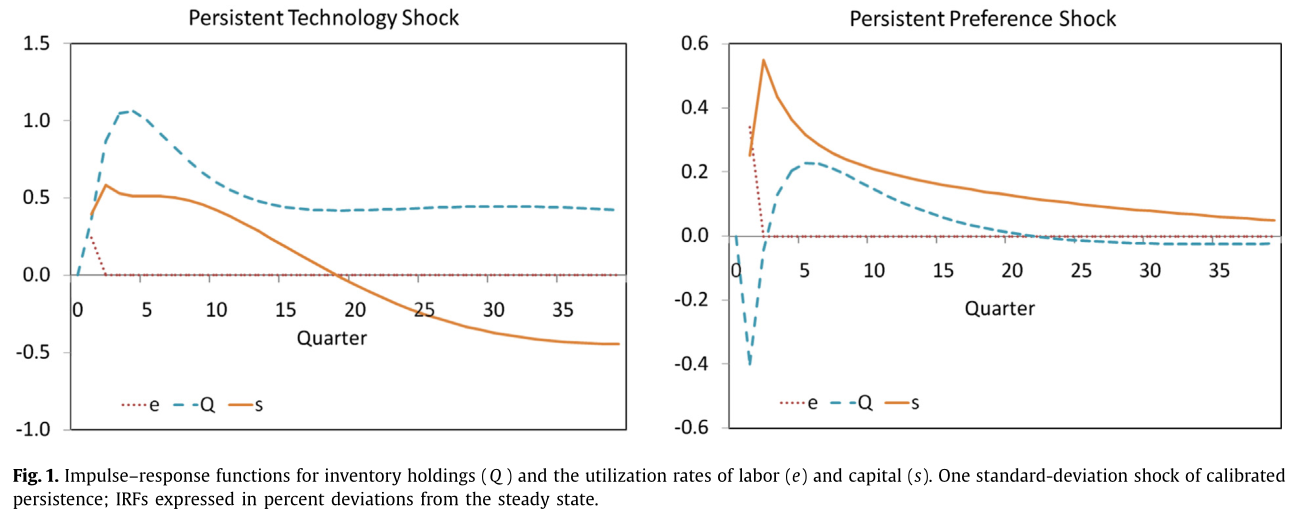
\includegraphics[scale=0.45]{table/fig1.png}
         \end{center}
       \end{figure}
    \begin{itemize}
    \item Inventory holdings and the two rates of capacity utilization increase at impact in response to, say, expansionary technology shock.
    \item In response to expansionary preference (demand) shocks, the economy will use capacity more intensively, while inventories fall at impact.
    \end{itemize}
\end{frame}

%----------------------------------------------------------------------------------------
\begin{frame}{Impulse–response analysis}
    \begin{multicols}{2}
		\begin{figure}
			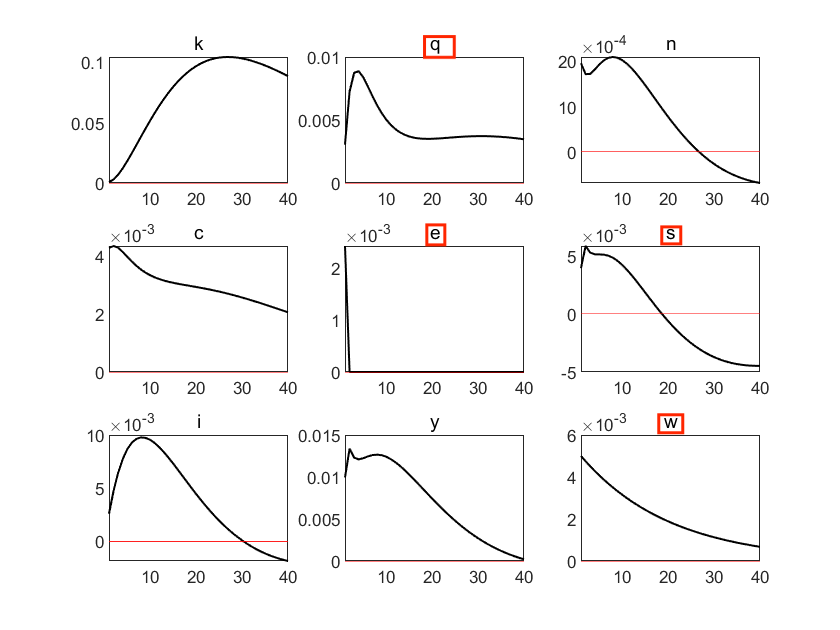
\includegraphics[scale=0.22]{table/s_fig_tec.png}
            \caption*{Persistent Technology Shock}
			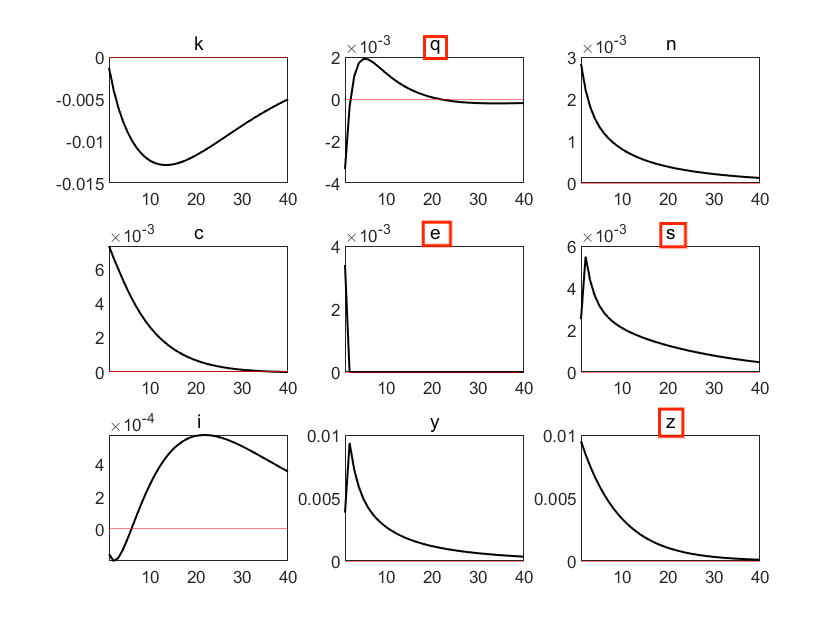
\includegraphics[scale=0.22]{table/s_fig_pre.png}
            \caption*{Persistent Preference Shock}
		\end{figure}
	\end{multicols}

\end{frame}

%----------------------------------------------------------------------------------------
\begin{frame}{Impulse–response analysis}
    \begin{figure}
         \begin{center}
         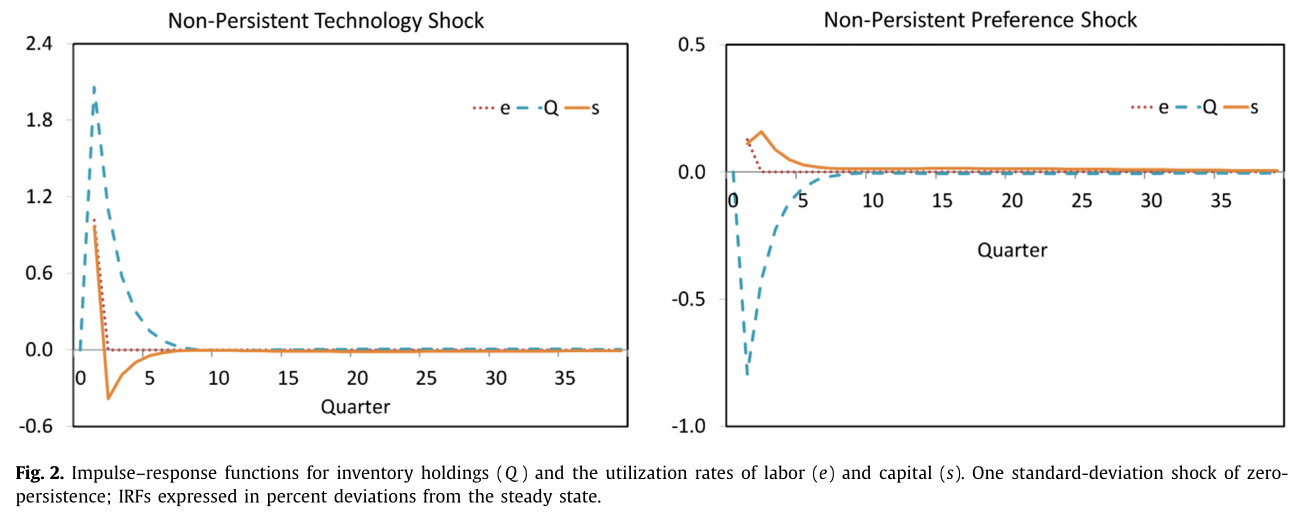
\includegraphics[scale=0.5]{table/fig2.png}
         \end{center}
    \end{figure}
    \begin{itemize}
    \item Temporary technology shocks emphasize inventory's consumption complement.
    \item Temporary demand shock emphasizes inventory's shock absorber role.
    \end{itemize}
\end{frame}

%----------------------------------------------------------------------------------------
\begin{frame}{Impulse–response analysis}
    \begin{multicols}{2}
		\begin{figure}
			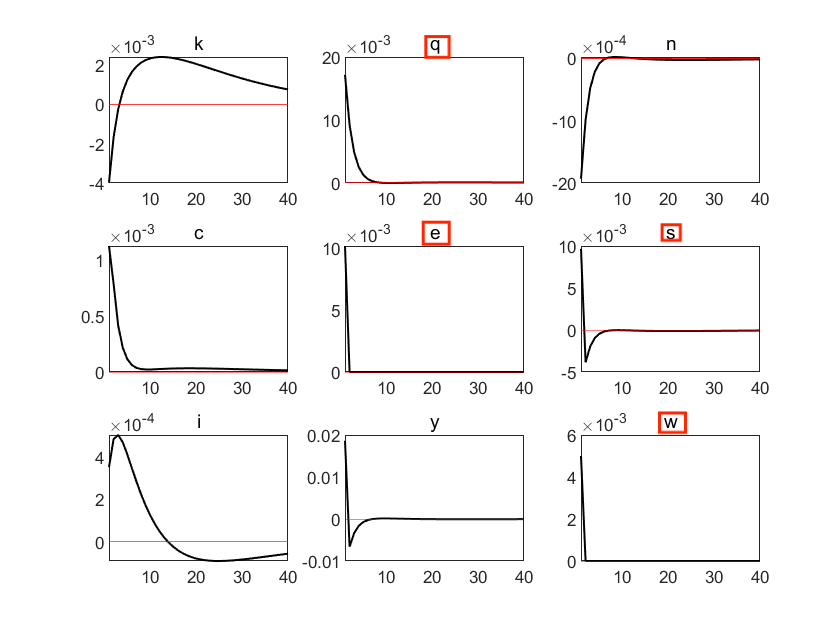
\includegraphics[scale=0.22]{table/s_fig_tec_non.png}
            \caption*{Non-Persistent Technology Shock}
			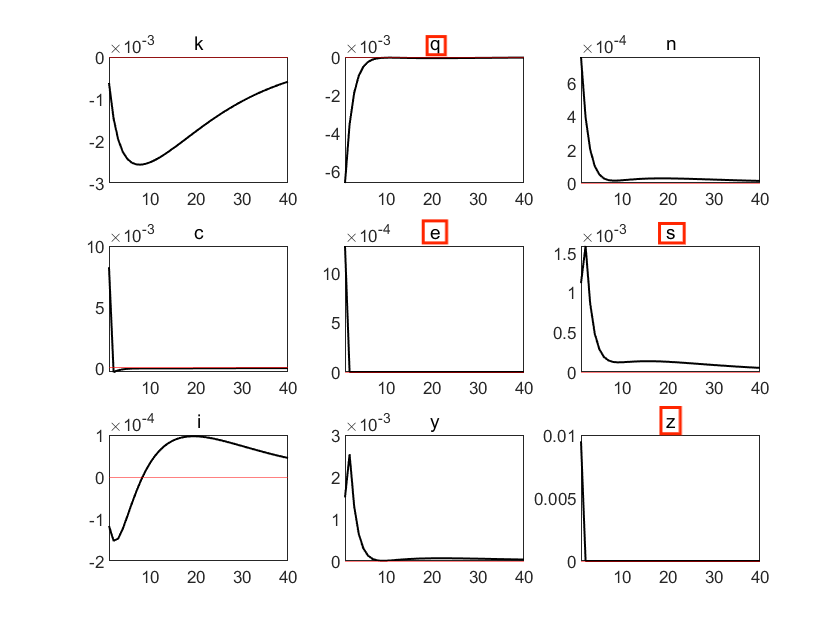
\includegraphics[scale=0.22]{table/s_fig_pre_non.png}
            \caption*{Non-Persistent Preference Shock}
		\end{figure}
	\end{multicols}
\end{frame}

%----------------------------------------------------------------------------------------
\begin{frame}{Impulse–response analysis}
    \begin{figure}
         \begin{center}
         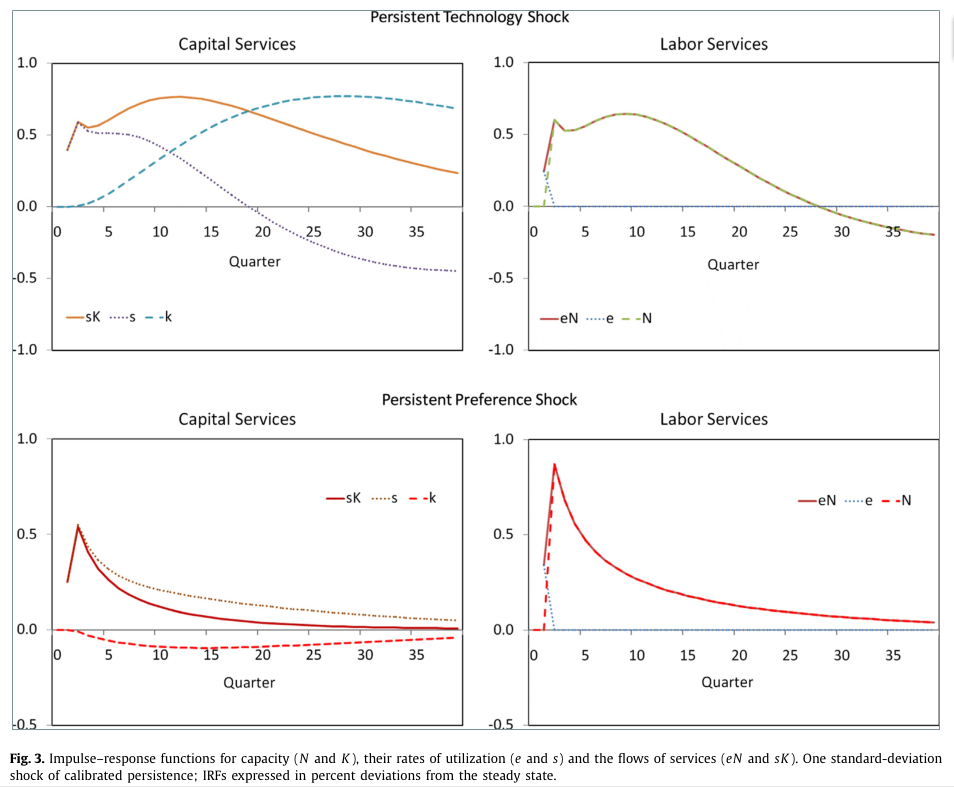
\includegraphics[width = 8cm]{table/fig3.png}
         \end{center}
    \end{figure}
\end{frame}

%----------------------------------------------------------------------------------------
\begin{frame}{Comparison to actual data}
	\begin{figure}
		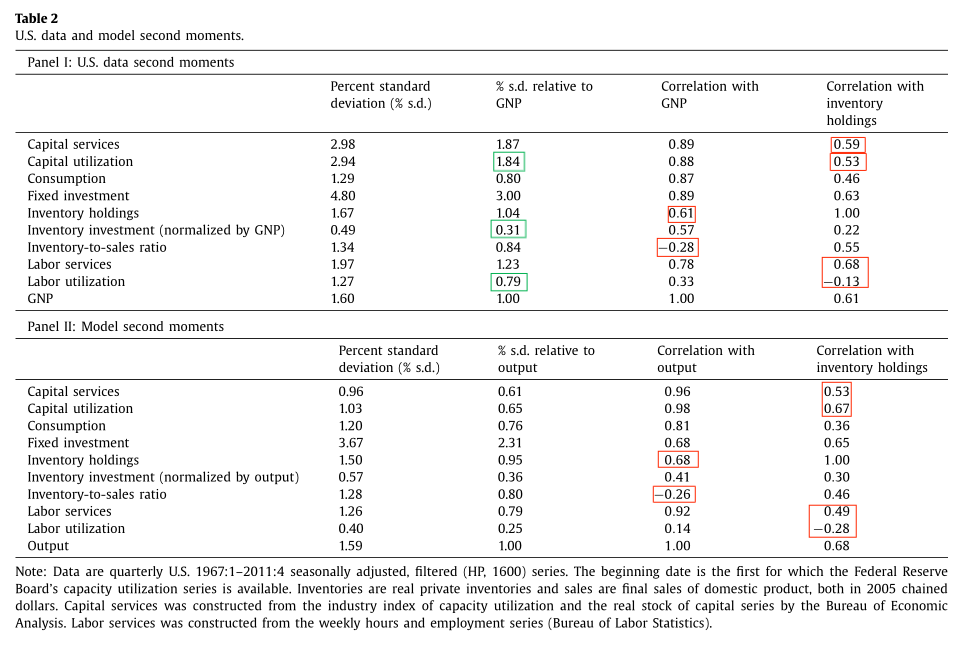
\includegraphics[width=11cm,height=6.5cm]{table/tab2.png}
	\end{figure}
\end{frame}

%----------------------------------------------------------------------------------------
\begin{frame}{The source of uncertainty and the persistence of the shocks}
	\begin{figure}
		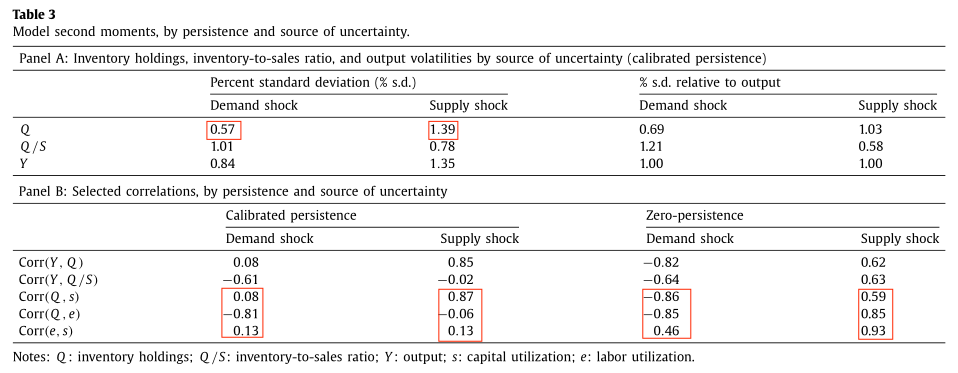
\includegraphics[width=13cm]{table/tab3.png}
	\end{figure}
\end{frame}

%----------------------------------------------------------------------------------------
\begin{frame}{The implications of inventories and capacity utilization}
	\begin{figure}
		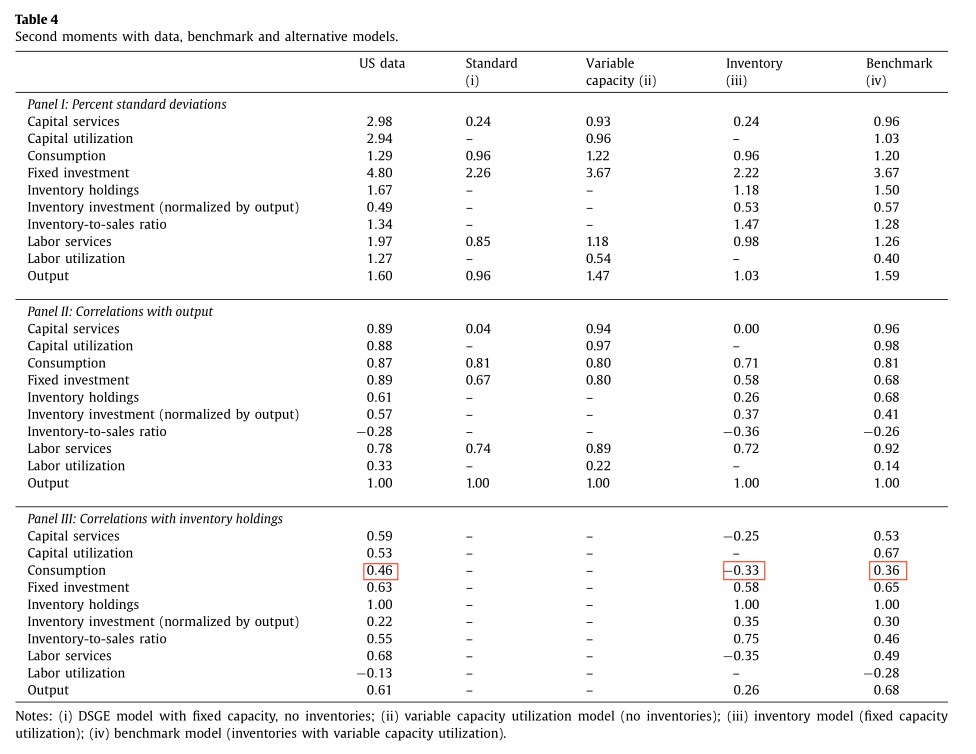
\includegraphics[width=12cm,height=6.5cm]{table/tab4.png}
	\end{figure}
\end{frame}

%----------------------------------------------------------------------------------------
\begin{frame}{The role of investment adjustment costs for the inventory}
	\begin{figure}
		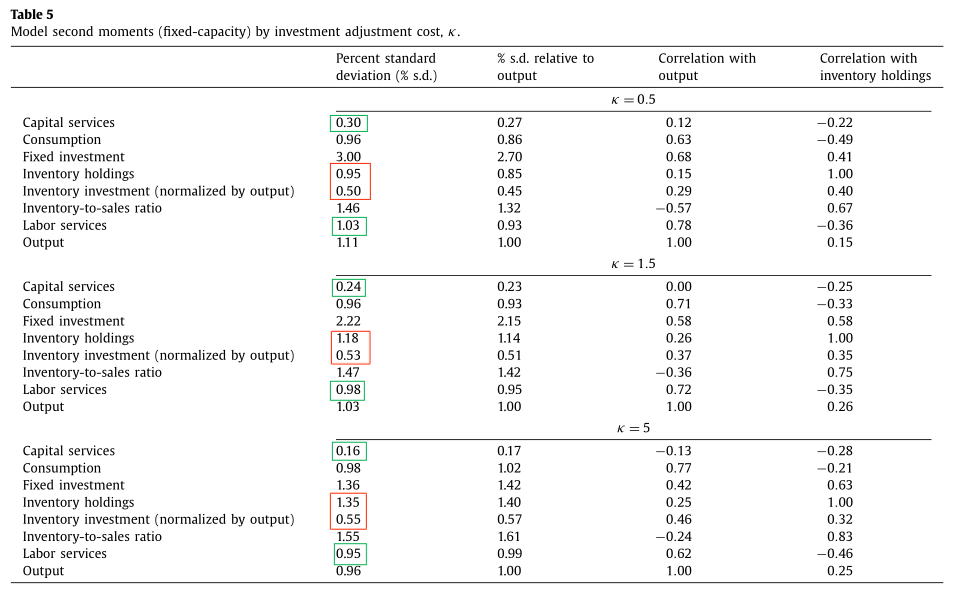
\includegraphics[width=11cm,height=6.5cm]{table/tab5.png}
	\end{figure}
\end{frame}

%----------------------------------------------------------------------------------------
\section{Concluding remarks}
%----------------------------------------------------------------------------------------
\begin{frame}{Conclusion}
    \begin{center}
      \begin{itemize}
      \vspace{8pt} %垂直间距
      \item First, inventory and capital utilization are mostly complementary, while inventory and labor utilization are mostly substitutes.
      \vspace{8pt}
      \item Second, temporary demand shocks emphasize the role of inventories as being a “shock absorber,” whereas high-persistence demand shocks, as well as technology shocks of any persistence, emphasize the role of inventories as being a complement to consumption.
      \vspace{8pt}
      \item Finally, we have discussed the role of investment adjustment costs on the dynamics of inventories.
    \end{itemize}
    \end{center}
\end{frame}


\end{document}
